% Options for packages loaded elsewhere
\PassOptionsToPackage{unicode}{hyperref}
\PassOptionsToPackage{hyphens}{url}
%
\documentclass[
  12pt,
]{article}
\title{Air Quality in Ukraine post Ukraine-Russia Dispute}
\usepackage{etoolbox}
\makeatletter
\providecommand{\subtitle}[1]{% add subtitle to \maketitle
  \apptocmd{\@title}{\par {\large #1 \par}}{}{}
}
\makeatother
\subtitle{Web address for GitHub repository}
\author{Shirley Fontanié, Rachel Gordon, and Julia Weinberg}
\date{}

\usepackage{amsmath,amssymb}
\usepackage{lmodern}
\usepackage{iftex}
\ifPDFTeX
  \usepackage[T1]{fontenc}
  \usepackage[utf8]{inputenc}
  \usepackage{textcomp} % provide euro and other symbols
\else % if luatex or xetex
  \usepackage{unicode-math}
  \defaultfontfeatures{Scale=MatchLowercase}
  \defaultfontfeatures[\rmfamily]{Ligatures=TeX,Scale=1}
  \setmainfont[]{Times New Roman}
\fi
% Use upquote if available, for straight quotes in verbatim environments
\IfFileExists{upquote.sty}{\usepackage{upquote}}{}
\IfFileExists{microtype.sty}{% use microtype if available
  \usepackage[]{microtype}
  \UseMicrotypeSet[protrusion]{basicmath} % disable protrusion for tt fonts
}{}
\makeatletter
\@ifundefined{KOMAClassName}{% if non-KOMA class
  \IfFileExists{parskip.sty}{%
    \usepackage{parskip}
  }{% else
    \setlength{\parindent}{0pt}
    \setlength{\parskip}{6pt plus 2pt minus 1pt}}
}{% if KOMA class
  \KOMAoptions{parskip=half}}
\makeatother
\usepackage{xcolor}
\IfFileExists{xurl.sty}{\usepackage{xurl}}{} % add URL line breaks if available
\IfFileExists{bookmark.sty}{\usepackage{bookmark}}{\usepackage{hyperref}}
\hypersetup{
  pdftitle={Air Quality in Ukraine post Ukraine-Russia Dispute},
  pdfauthor={Shirley Fontanié, Rachel Gordon, and Julia Weinberg},
  hidelinks,
  pdfcreator={LaTeX via pandoc}}
\urlstyle{same} % disable monospaced font for URLs
\usepackage[margin=2.54cm]{geometry}
\usepackage{longtable,booktabs,array}
\usepackage{calc} % for calculating minipage widths
% Correct order of tables after \paragraph or \subparagraph
\usepackage{etoolbox}
\makeatletter
\patchcmd\longtable{\par}{\if@noskipsec\mbox{}\fi\par}{}{}
\makeatother
% Allow footnotes in longtable head/foot
\IfFileExists{footnotehyper.sty}{\usepackage{footnotehyper}}{\usepackage{footnote}}
\makesavenoteenv{longtable}
\usepackage{graphicx}
\makeatletter
\def\maxwidth{\ifdim\Gin@nat@width>\linewidth\linewidth\else\Gin@nat@width\fi}
\def\maxheight{\ifdim\Gin@nat@height>\textheight\textheight\else\Gin@nat@height\fi}
\makeatother
% Scale images if necessary, so that they will not overflow the page
% margins by default, and it is still possible to overwrite the defaults
% using explicit options in \includegraphics[width, height, ...]{}
\setkeys{Gin}{width=\maxwidth,height=\maxheight,keepaspectratio}
% Set default figure placement to htbp
\makeatletter
\def\fps@figure{htbp}
\makeatother
\setlength{\emergencystretch}{3em} % prevent overfull lines
\providecommand{\tightlist}{%
  \setlength{\itemsep}{0pt}\setlength{\parskip}{0pt}}
\setcounter{secnumdepth}{5}
\ifLuaTeX
  \usepackage{selnolig}  % disable illegal ligatures
\fi

\begin{document}
\maketitle

\newpage
\tableofcontents 
\newpage
\listoftables 
\newpage
\listoffigures 
\newpage

\hypertarget{rationale-and-research-questions}{%
\section{Rationale and Research
Questions}\label{rationale-and-research-questions}}

\begin{quote}
{[}Rachel to do{]}
\end{quote}

\newpage

\hypertarget{dataset-information}{%
\section{Dataset Information}\label{dataset-information}}

\begin{quote}
Describe sources of data here (input Julia paragraph)
\end{quote}

\begin{quote}
Explain data wrangling process here (shirley do this)
\end{quote}

\begin{longtable}[]{@{}ll@{}}
\toprule
Data File Name & Description \\
\midrule
\endhead
UkraineData & (Raw) Ukraine air quality data \\
Ukraine\_Processed & (Processed) Ukraine air quality data, w/o na's \\
Dnipro\_2021 & Dnipro PM2.5 + PM10, Mar 2021 \\
Dnipro\_2022 & Dnipro PM2.5+ PM10, Mar 2022 \\
Lviv\_2021 & Lviv PM 2.5 + PM10, Mar 2021 \\
Lviv\_2022 & Lviv PM 2.5 + PM10, Mar 2022 \\
FULL\_DNIPRO & Lviv\_2021 + Lviv\_2022 combined \\
FULL\_LVIV & Dnipro\_2021 + Dnipro\_2022 combined \\
FULL\_Air\_quality & 2022 Air Quality for Lviv and Dnipro \\
Full-air\_quality\_21\_22 & 2021 and 2022 Data for Lviv and Dnipro \\
\bottomrule
\end{longtable}

\newpage

\hypertarget{exploratory-analysis}{%
\section{Exploratory Analysis}\label{exploratory-analysis}}

\begin{quote}
INSERT COMMENTARY ABOUT EXPLORATORY ANALYSIS COMPONENTS
\end{quote}

\begin{figure}
\centering
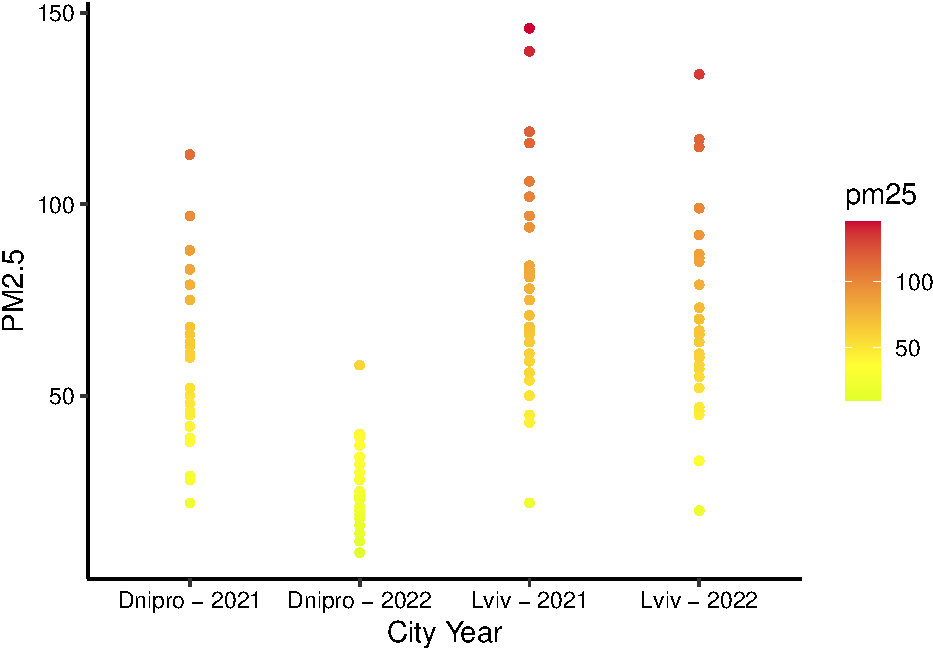
\includegraphics{Fontanie_Gordon_Weinberg_Project_files/figure-latex/plot of PM25air pollution levels by CityYear-1.pdf}
\caption{PM2.5 Distribution}
\end{figure}

\hfill\break

\begin{longtable}[]{@{}lrrrr@{}}
\caption{PM2.5 Levels by City}\tabularnewline
\toprule
City & Mean & Min & Max & Std Dev \\
\midrule
\endfirsthead
\toprule
City & Mean & Min & Max & Std Dev \\
\midrule
\endhead
Dnipro & 49.41546 & 4 & 160 & 25.91608 \\
Lviv & 60.51086 & 8 & 518 & 34.79405 \\
\bottomrule
\end{longtable}

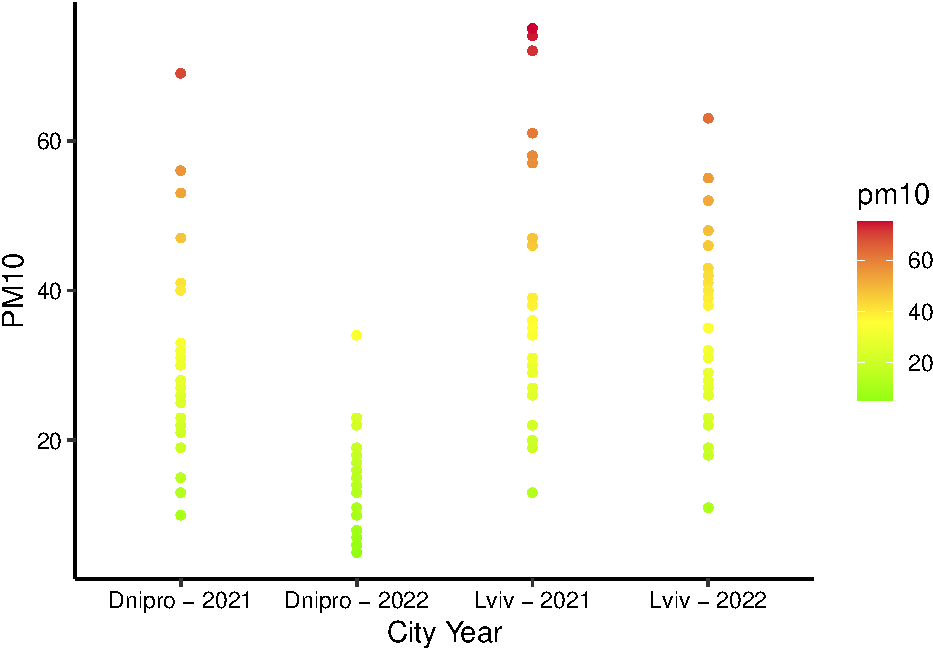
\includegraphics{Fontanie_Gordon_Weinberg_Project_files/figure-latex/plot of PM10 levels by CityYear-1.pdf}\\

\begin{longtable}[]{@{}lrrrr@{}}
\caption{PM10 Levels by City}\tabularnewline
\toprule
City & Mean & Min & Max & Std Dev \\
\midrule
\endfirsthead
\toprule
City & Mean & Min & Max & Std Dev \\
\midrule
\endhead
Dnipro & 24.73309 & 2 & 120 & 15.82186 \\
Lviv & 30.29246 & 4 & 606 & 26.78330 \\
\bottomrule
\end{longtable}

\newpage

\hypertarget{analysis}{%
\section{Analysis}\label{analysis}}

\hypertarget{question-1-are-there-significant-differences-in-air-quality-levels-between-affected-ukrainian-cities-during-the-russian-invasion}{%
\subsection{Question 1: Are there significant differences in air quality
levels between affected Ukrainian cities during the Russian
invasion?}\label{question-1-are-there-significant-differences-in-air-quality-levels-between-affected-ukrainian-cities-during-the-russian-invasion}}

\begin{quote}
{[}Shirley insert text about how we analyzed - visualizations and
statistical tests{]}
\end{quote}

\begin{quote}
\textbf{PM2.5 in Lviv and Dnipro during the invasions}
\end{quote}

\begin{figure}
\centering
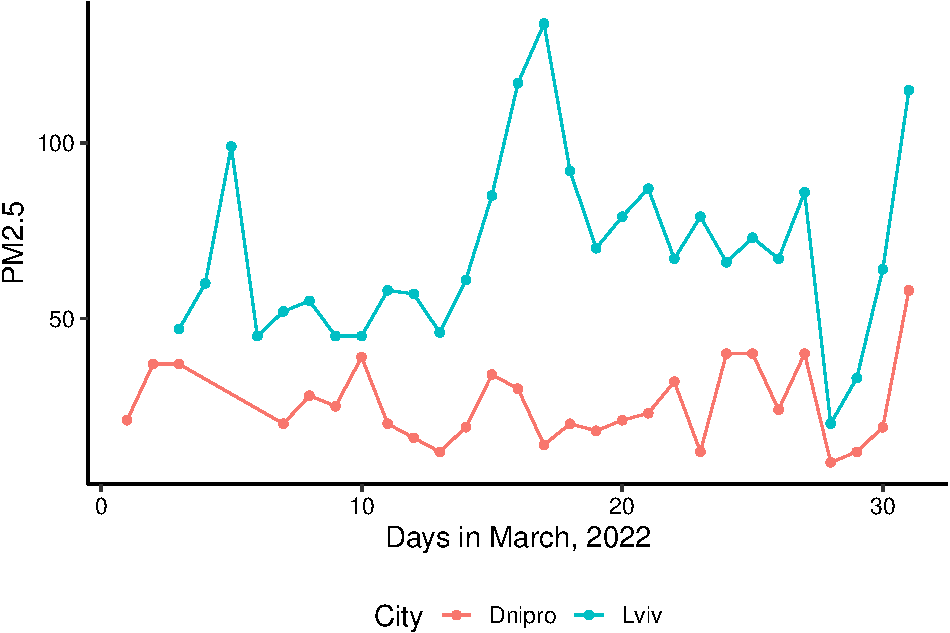
\includegraphics{Fontanie_Gordon_Weinberg_Project_files/figure-latex/Plotting Lviv vs Dnipro PM25-1.pdf}
\caption{2022 PM2.5 Levels in Dnipro and Lviv}
\end{figure}

\begin{figure}
\centering
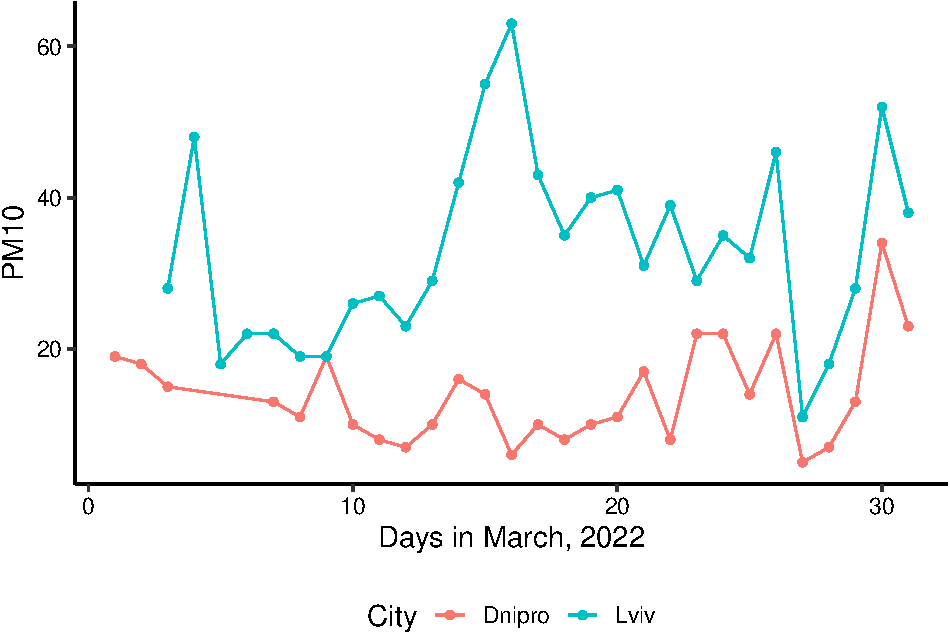
\includegraphics{Fontanie_Gordon_Weinberg_Project_files/figure-latex/Plotting Lviv and Dnipro PM10-1.pdf}
\caption{2022 PM10 Levels in Lviv and Dnipro}
\end{figure}

\newpage

\hypertarget{question-2-are-there-significant-differences-in-air-quality-levels-in-affected-ukrainian-cities-before-and-during-the-russian-attacks}{%
\subsection{Question 2: Are there significant differences in air quality
levels in affected Ukrainian cities before and during the Russian
attacks?}\label{question-2-are-there-significant-differences-in-air-quality-levels-in-affected-ukrainian-cities-before-and-during-the-russian-attacks}}

\begin{quote}
Similiar to our first research question, we conducted a visual analysis
of PM2.5 and PM10 levels within Dnipro and Lviv for years 2021 and 2022.
For each of our visualizations, we created line plots that showed the
air pollution levels within the city, comparing 2021 to 2022. As we
needed to visualize the levels of both PM2.5 and PM10, we created four
different plots - ``PM2.5 Levels in Dnipro'', ``PM2.5 Levels in Lviv'',
``PM10 Levels in Dnipro'', and ``PM10 Levels in Lviv''. Within each of
these plots, we also created annotations to indicate the specific dates
of the missile attacks within the cities to see if there were any PM2.5
or PM10 increases or decreases around those dates. Additionally, we
conducted a linear regression analysis for each of these charts to
understand if there is a significant difference in PM2.5 levels and PM10
levels within Dnipro and Lviv in March of 2021 compared to March of
2022.\\
\end{quote}

\begin{quote}
\textbf{PM2.5 in Dnipro}\\
When plotting PM2.5 levels in Dnipro in 2021 compared to 2022 (Figure
3), it is evident that overall, PM2.5 levels were higher in 2021 than
2022. It is also interesting to note that around March 11 in 2022, when
the missile attack occured, there appears to be an uptick in PM2.5
levels and then sharply decreases shortly after. Overall in both years,
there seems to be a variety of fluctuation in PM2.5 levels and they are
not consistent within each year. Additionally, within most of 2022,
PM2.5 levels stayed within ``good'' to ``moderate'' levels, with an
exception of reaching a level of ``unhealthy for sensitive groups'' at
the end of March 2022. In March 2021, however, the PM2.5 levels were
mainly in the ``unhealthy for sensitive groups'' or ``unhealthy''
category, with only a few days throughout that month in ``moderate''
levels.
\end{quote}

\begin{quote}
For the statistical analysis, we ran a linear regression model of pm2.5
levels by year within Dnipro, to understand if there are significant
differences in PM2.5 levels within the city in March 2021 compared to
March 2022. The linear regression showed the slope was negative
(-32.253), meaning that PM2.5 levels decreased in 2022 compared to 2021.
Additionally, the linear regression showed that the relationship between
PM2.5 levels and year in Dnipro is significant (p = 5.074e-10), meaning
that there is a significant difference in PM2.5 levels in Dnipro in 2022
compared to 2021.
\end{quote}

\begin{figure}
\centering
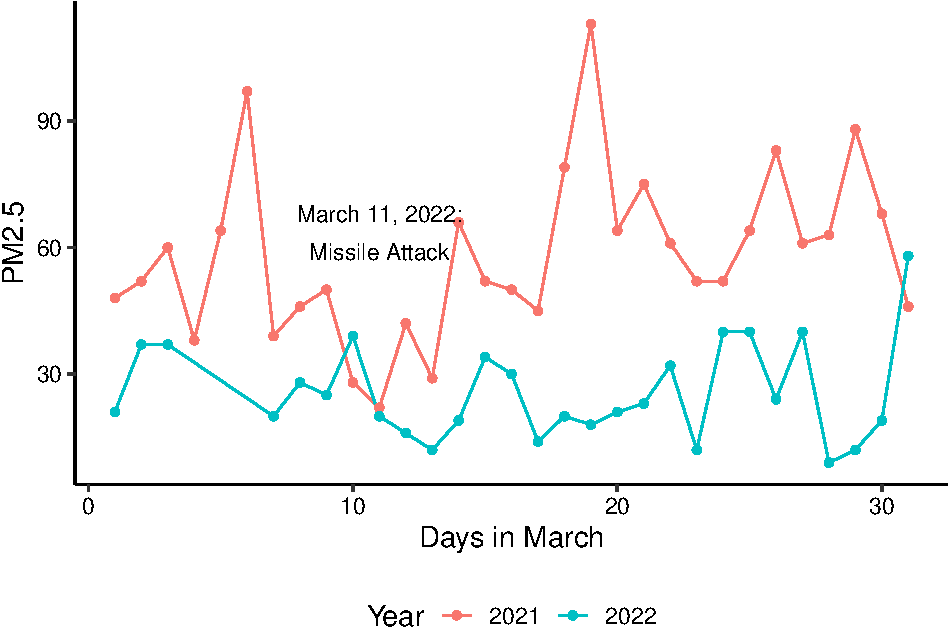
\includegraphics{Fontanie_Gordon_Weinberg_Project_files/figure-latex/Visualizing PM25 in Dnipro-1.pdf}
\caption{PM2.5 Levels in Dnipro}
\end{figure}

\newpage

\begin{quote}
\textbf{PM2.5 in Lviv}\\
When plotting PM2.5 levels in Lviv in 2021 compared to 2022 (Figure 4),
there is no clear difference in levels between years. It is interesting
to note that before the March 18 attack, PM2.5 levels were increasing,
and after the March 18, 2022 missile attack, it appears levels sharply
decreased. Overall in both years, it appears that there seems to be a
variety of fluctuation in PM2.5 in Lviv. Additionally, within both 2021
and 2022, it is very rare that levels are within the ``good'' range of
PM2.5 (\textless15.4) and are typically within ``moderate'' to
``unhealthy'' levels.
\end{quote}

\begin{quote}
For the statistical analysis, we ran a linear regression model of PM2.5
levels by year within Lviv, to understand if there are significant
differences in levels within the city in March 2021 compared to March
2022. Through the analysis, we found that the slope was negative
(-10.284), meaning that PM2.5 levels decreased in 2022 compared to 2021.
However, the linear regression showed that the negative relationship
between PM2.5 levels and year in Lviv is not significant (p=0.1639).
\end{quote}

\begin{figure}
\centering
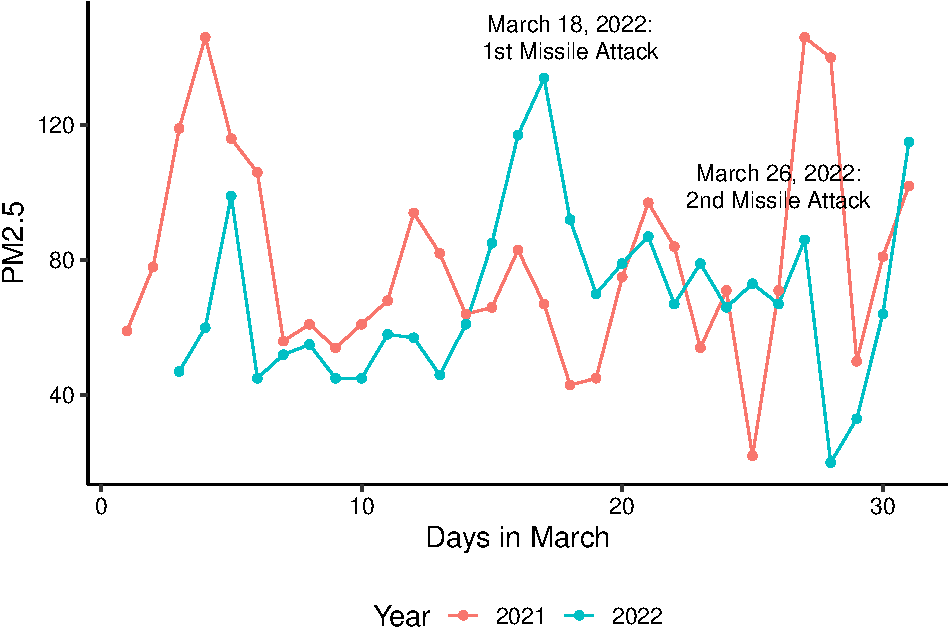
\includegraphics{Fontanie_Gordon_Weinberg_Project_files/figure-latex/visualizing PM25 in Lviv-1.pdf}
\caption{PM2.5 Levels in Lviv}
\end{figure}

\newpage

\begin{quote}
\textbf{PM10 in Dnipro}\\
When plotting PM10 levels in Dnipro in 2021 compared to 2022 (Figure 5),
it is evident that overall, PM10 levels were higher in 2021 compared to
2022. When looking at the PM10 levels around the March 11 attack in
2022, there does not appear to be a significant increase. Additionally,
in March 2022, PM10 levels seemed to stay within or below ``moderate''
levels, whereas 2021 levels ranged from ``moderate'' to ``unhealthy for
sensitive groups''.
\end{quote}

\begin{quote}
For the statistical analysis, we ran a linear regression of PM10 levels
by year within Dnipro, to understand if there are significant
differences in levels within the city in March 2021 compared to March
2022. Through the analysis, we found that the slope was negative
(-15.677), meaning that PM10 levels decreased in 2022 compared to 2021.
Additionally, the linear regression showed that these results are
statistically significant (p=4.325e-07), meaning there is a significant
difference in PM10 levels in Dnipro in 2022 compared to 2021.
\end{quote}

\begin{figure}
\centering
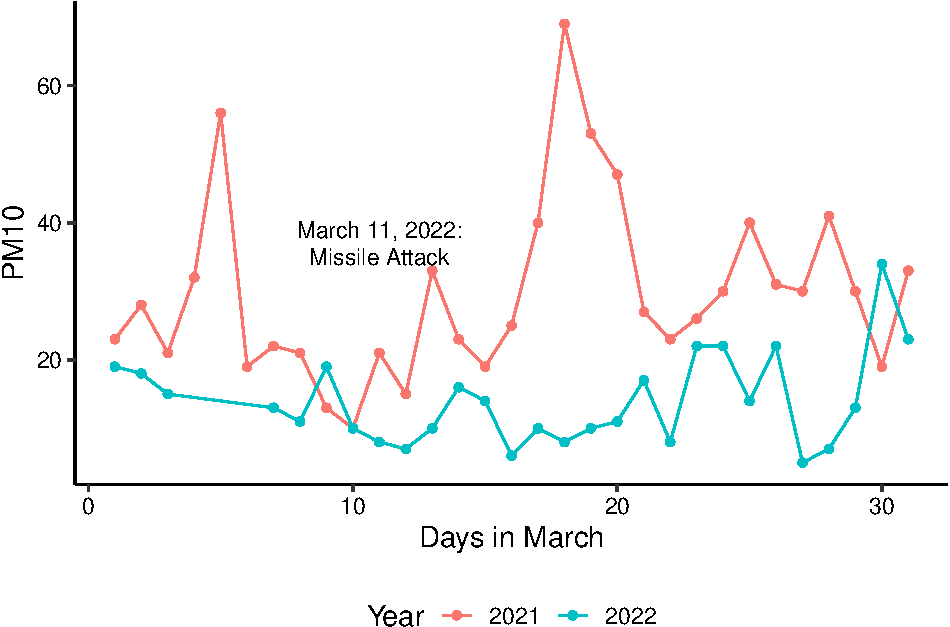
\includegraphics{Fontanie_Gordon_Weinberg_Project_files/figure-latex/visualizing PM10 in Dnipro-1.pdf}
\caption{PM10 Levels in Dnipro}
\end{figure}

\newpage

\begin{quote}
\textbf{PM10 in Lviv}\\
When plotting PM10 levels in Lviv in 2021 compared to 2022 (Figure 6),
there is no clear difference observed in PM10 levels between the years.
It is also interesting to note that there does not seem to a significant
change in PM10 levels after the March 18 attack, and PM10 levels appear
to sharply drop after the March 26 attack. Additionally, PM10 levels in
both years stay mainly within ``unhealthy for sensitive groups'' to
``good'' levels, but at some points in 2021, levels reach into the
``unhealthy'' level.
\end{quote}

\begin{quote}
For the statistical analysis, we ran a linear regression of PM10 levels
by year within Lviv, to understand if there are significant differences
in levels within the city in March 2021 compared to March 2022. Through
the analysis, we found that the slope was negative (-5.673), meaning
that PM10 levels decreased in 2022 compared to 2021 in Lviv. However,
the linear regression showed that these results are not statistically
significant (p=0.1364), meaning that there is not a significant
difference in PM10 levels in Lviv in 2022 compared to 2021.
\end{quote}

\begin{figure}
\centering
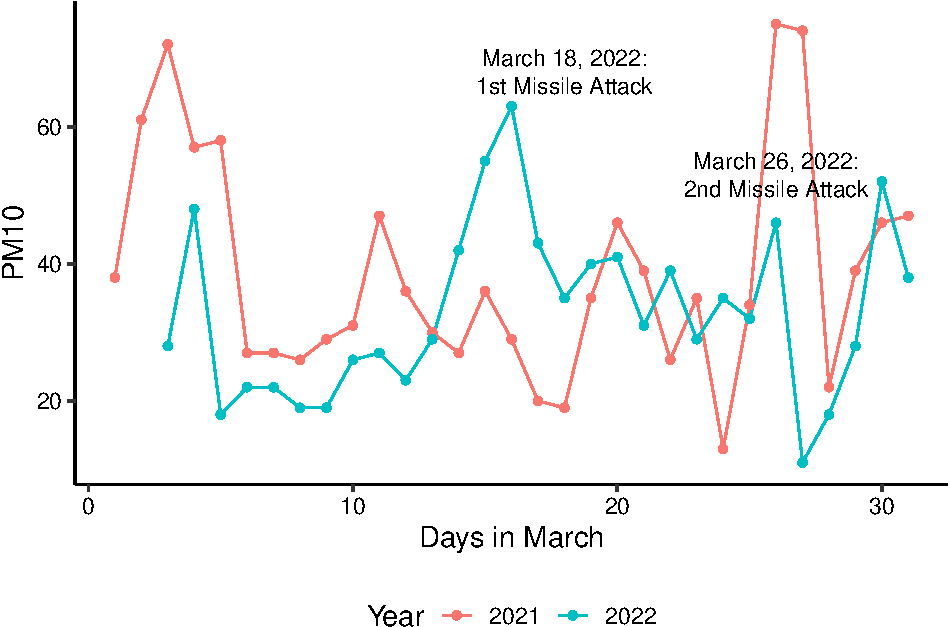
\includegraphics{Fontanie_Gordon_Weinberg_Project_files/figure-latex/visualizing PM10 in Lviv-1.pdf}
\caption{PM10 Levels in Lviv}
\end{figure}

\newpage

\hypertarget{summary-and-conclusions}{%
\section{Summary and Conclusions}\label{summary-and-conclusions}}

\hypertarget{question-1-are-there-significant-differences-in-air-quality-levels-between-affected-ukrainian-cities-during-the-russian-invasion-1}{%
\subsection{Question 1: Are there significant differences in air quality
levels between affected Ukrainian cities during the Russian
invasion?}\label{question-1-are-there-significant-differences-in-air-quality-levels-between-affected-ukrainian-cities-during-the-russian-invasion-1}}

\begin{quote}
{[}Shirley insert results from our analysis{]}
\end{quote}

\hypertarget{question-2-are-there-significant-differences-in-air-quality-levels-in-affected-ukrainian-cities-before-and-during-the-russian-attacks-1}{%
\subsection{Question 2: Are there significant differences in air quality
levels in affected Ukrainian cities before and during the Russian
attacks?}\label{question-2-are-there-significant-differences-in-air-quality-levels-in-affected-ukrainian-cities-before-and-during-the-russian-attacks-1}}

\begin{quote}
There were significant differences in both PM2.5 and PM10 levels in
Dnipro in March of 2022 compared to March of 2021. However, there were
no significant differences in PM2.5 and PM10 levels in Lviv in March of
2022 compared to March of 2021. In Dnipro in March of 2022, the PM2.5
levels were much higher in 2021 compared to 2022, which was surprising
given the context originally discussed in which air pollution tends to
increase during times of war due to explosions and infrastructure
collapse that increase levels of hazardous dust and debris.
\end{quote}

\begin{quote}
As Dnipro typically has a high presence of industrial activity during
pre-war times, it is possible that PM2.5 and PM10 levels decreased due
to the industrial sector activities being paused during the war.
Additionally, since Lviv is more of a cultural city and does not have a
heavy industrial presence, it is likely that PM2.5 levels and PM10
levels didn't significantly change if industrial activity is a more
influential factor than presence of missile attacks. This is an
interesting idea that would be valuable to explore in future studies,
comparing multiple cities that have experienced missile attacks with
varying industrial profiles and identifying if air pollution levels
change in those cities if industrial activity is paused due to war.
\end{quote}

\begin{quote}
\textbf{Limitations}\\
It is important to note that our study was limited in the amount of data
analyzed over time. To improve the analysis, if it's possible to find
more data, we would study PM2.5 and PM10 levels from at least three
years prior. Additionally, depending on how the war continues, it would
be interested to study air pollution levels beyond March of 2022,
especially if the war worsens and there is an increasing amount of
missile attacks. Our study is also limited in the number of cities
analyzed. To improve the study, we would expand our analysis to more
cities throughout Ukraine if it is possible to find the data.
\end{quote}

\begin{quote}
Additionally, it may be valuable to explore other variables that may be
affecting air pollution levels besides war presence and missile attacks.
Specifically, population and population density may have an impact on
air pollution levels. As it was found that Lviv had much higher absolute
levels of air pollution compared to Dnipro, it would be valuable to
understand differences in population, population density, and tourism
activity (as Lviv is the cultural capital of the country) has any impact
on air pollution levels.
\end{quote}

\begin{quote}
\textbf{Conclusions}\\
From this study, we can conclude that there were differences in air
quality levels between affected cities during the Russian invasion.
However, we cannot conclude that varying levels of missile attacks is
the only factor contributing to these differences. Additionally, we can
conclude that cities may differ in air pollution levels during the
presence of war activity compared to before, however, it appears that
missile attacks may have a negative relationship with air pollution
levels. These results show that there may be other variables affecting
air pollution levels in cities (such as the presence or absence of
industrial activity) that would be valuable to analyze in future
studies.
\end{quote}

\newpage

\hypertarget{references}{%
\section{References}\label{references}}

\textless add references here if relevant, otherwise delete this
section\textgreater{}

\end{document}
